\subsection{Masking}

\begin{margintable}
    \centering
    \caption[IoU of masks generated by EntropyMasker, Improved FESI, and FESI]{
        Intersection over Union (IoU) with \qty{95}{\percent} CI for three pathology masking algorithms applied to HHG overview images.
    }
    \label{tab:masking}
    \begin{tabular}[\linewidth]{cc}
        \toprule
        Algorithm & IoU \\
        \midrule
        FESI & \num{0.64 \pm 0.07} \\
        Improved FESI & \num{0.64 \pm 0.14} \\
        EntropyMasker & \textbf{\num{0.92 \pm 0.06}} \\
        \bottomrule
    \end{tabular}
\end{margintable}

FESI, Improved FESI, and EntropyMasker have been evaluated against 8 manually masked HHG overview images.
\Cref{fig:masking-results} shows the binary masks created by the algorithms.
The mean IoU for every algorithm is reported in \cref{tab:masking}.
EntropyMasker masks HHG overview images significantly better than (Improved) FESI.

\begin{figure*}
    \centering
    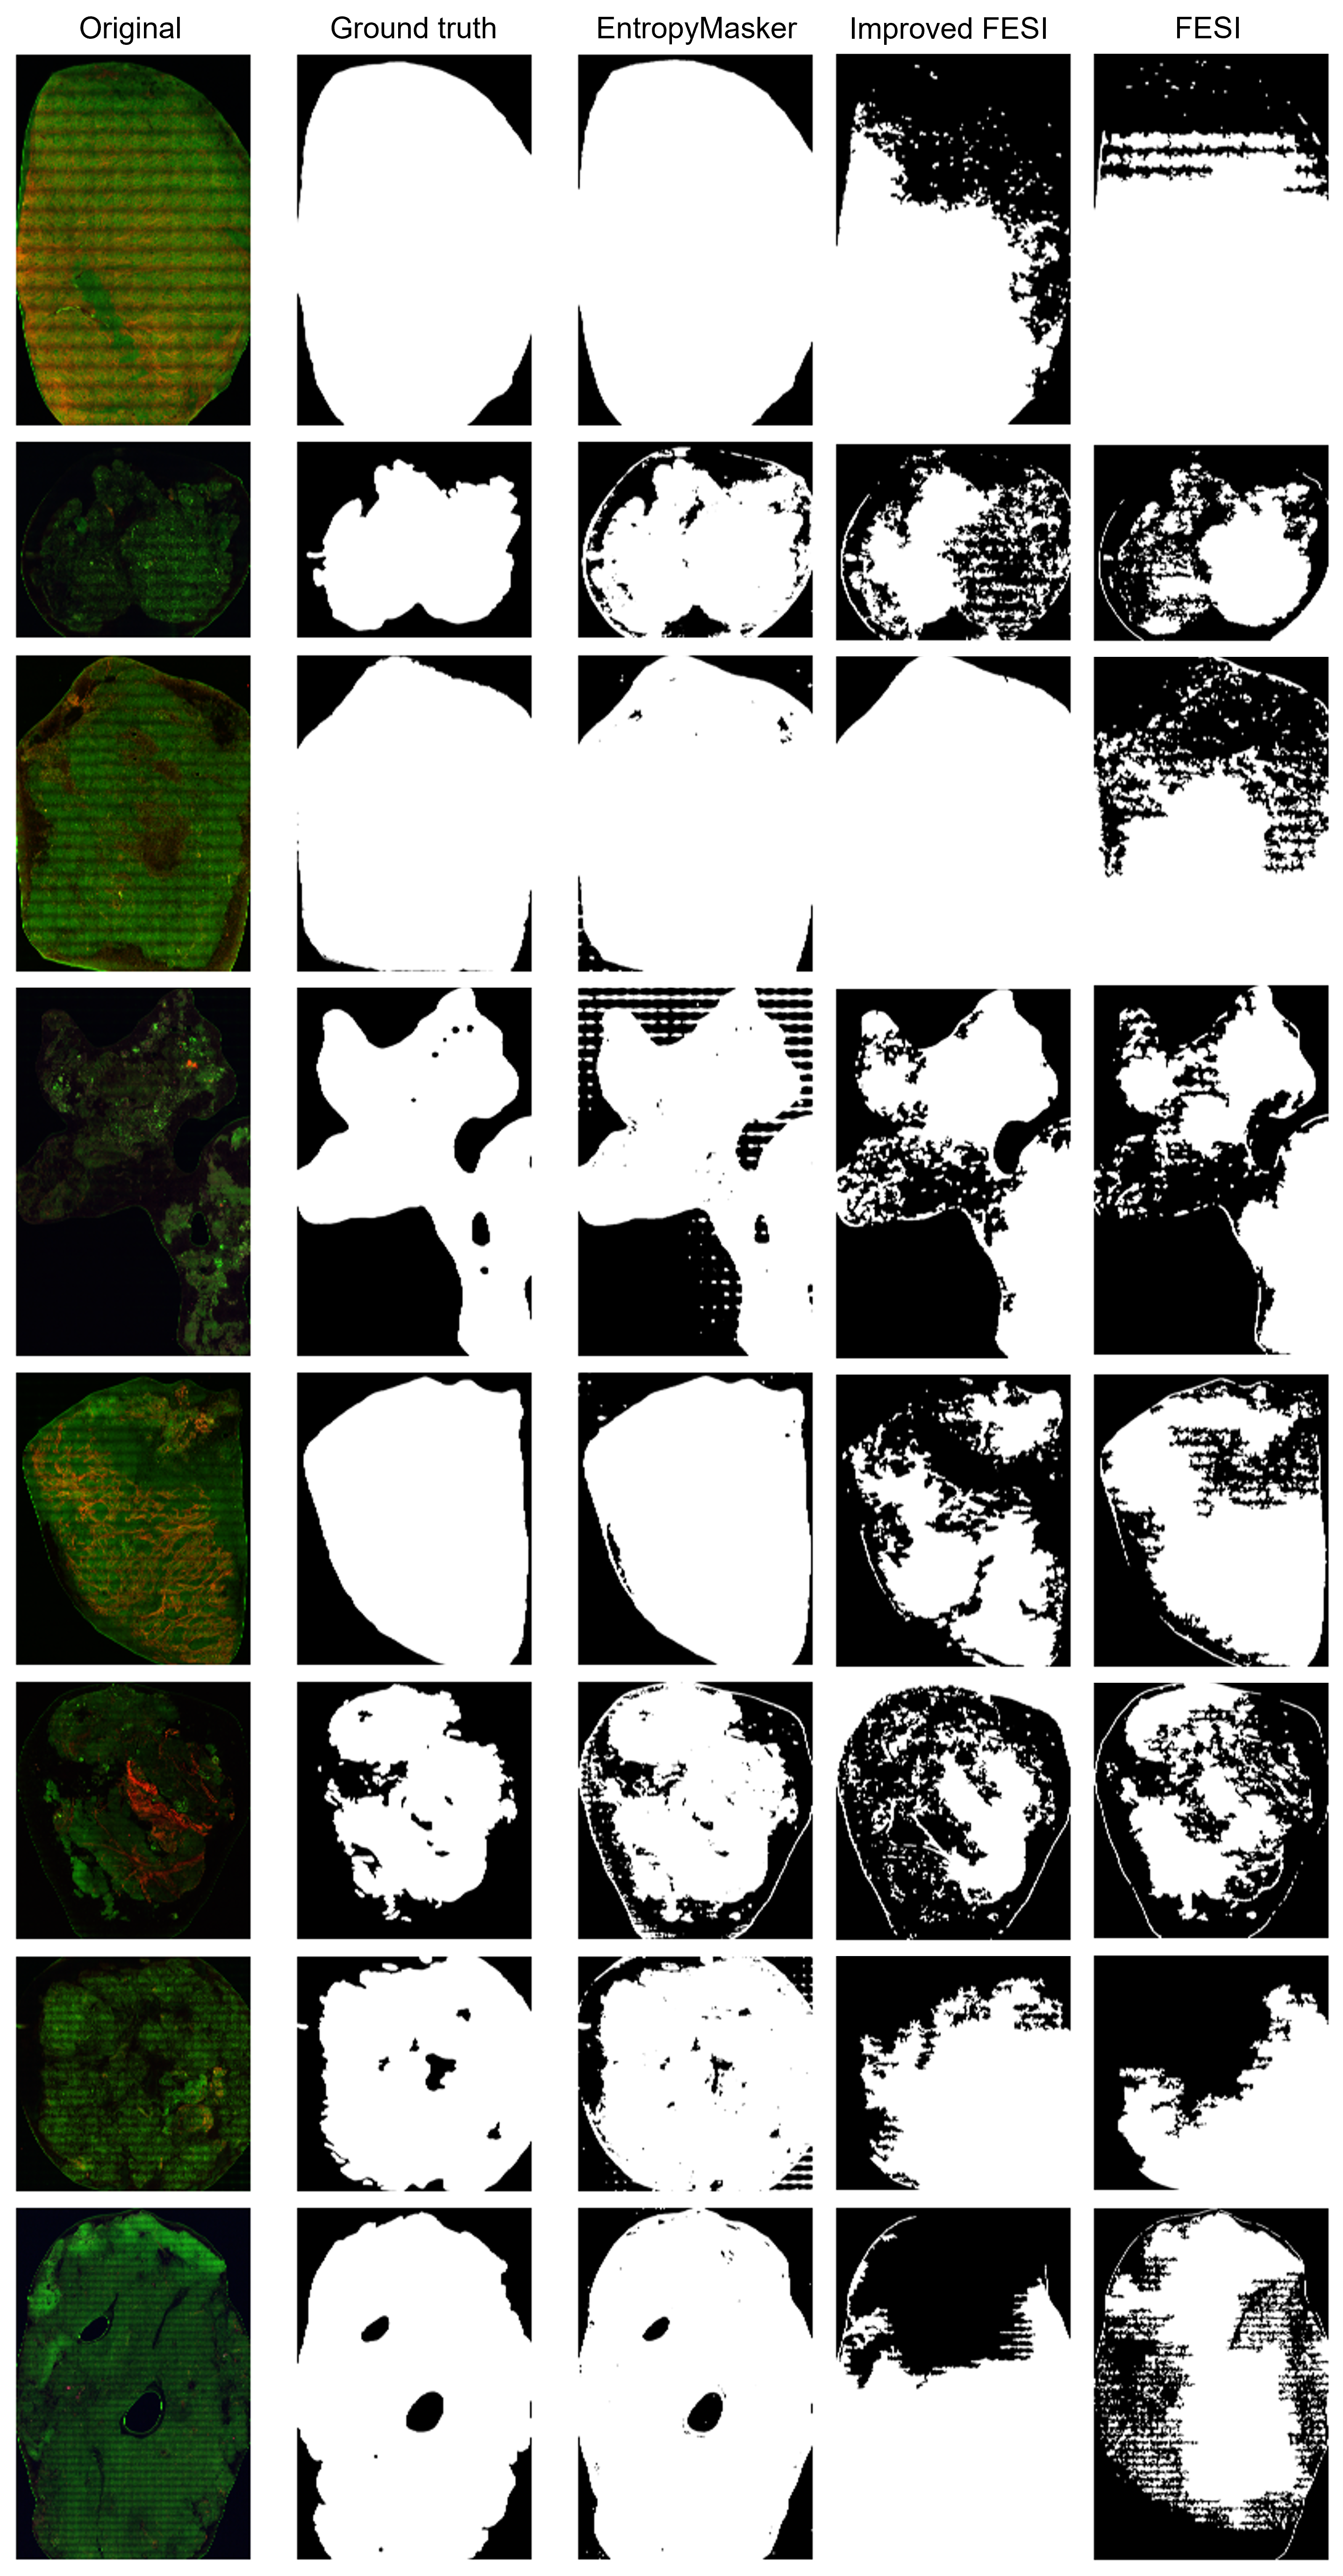
\includegraphics[width=\linewidth]{pediatric-brain-tumours/images/masking.png}
    \caption[Masks generated by EntropyMasker, Improved FESI, and FESI]{
        Masks generated by EntropyMasker, Improved FESI, and FESI on HHG overview images.
        The first two columns show the original images and the ground truth segmentation.
        The other columns show the generated masks.
    }
    \label{fig:masking-results}
\end{figure*}